\documentclass[11pt]{article}
\usepackage[margin=1in]{geometry}
\usepackage{amsmath,amssymb,amsthm}
\usepackage[vlined,linesnumbered]{algorithm2e}
\LinesNotNumbered
\usepackage{enumitem}
\usepackage{tikz}
\usetikzlibrary{arrows.meta, positioning}

\setlength{\parindent}{0pt}
\setlength{\parskip}{0.5em}

\begin{document}


\section*{1. Checking Correctness}

\vspace{-10pt}
\subsection*{Algorithm}

\begin{center}
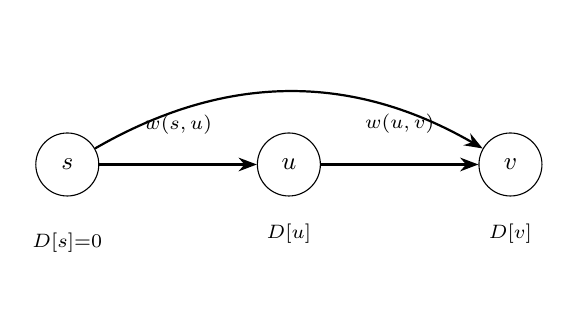
\begin{tikzpicture}[>=Stealth, node distance=2cm, every node/.style={circle, draw, minimum size=8mm, inner sep=1pt, font=\small}]
\node (s) {$s$};
\node[right=of s] (u) {$u$};
\node[right=of u] (v) {$v$};
\draw[->, thick] (s) -- node[above, draw=none, font=\scriptsize] {$w(s,u)$} (u);
\draw[->, thick] (u) -- node[above, draw=none, font=\scriptsize] {$w(u,v)$} (v);
\node[draw=none, below=2pt of s, font=\scriptsize] {$D[s]{=}0$};
\node[draw=none, below=2pt of u, font=\scriptsize] {$D[u]$};
\node[draw=none, below=2pt of v, font=\scriptsize] {$D[v]$};
\draw[->, thick, bend left=30] (s) to node[above, draw=none, font=\scriptsize] {} (v);
\end{tikzpicture}
\end{center}

Return \textbf{true} iff all three conditions hold:
\begin{enumerate}[leftmargin=*,itemsep=2pt]
\item $D[s] = 0$
\item $\forall\, (u,v) \in E$: \; $D[v] \le D[u] + w(u,v)$ \hfill (triangle inequality)
\item $\forall\, v \ne s$ with $D[v] < \infty$: \; $\exists\, (u,v) \in E$ with $D[v] = D[u] + w(u,v)$ \hfill (tightness)
\end{enumerate}

\vspace{-20pt}
\subsection*{Proof of correctness}

\textbf{Necessary:} Shortest distances satisfy (1)--(3) by definition.

\textbf{Sufficient ($D[v] = \mathrm{dist}(s,v)$ when (1)--(3) hold):}

\textbf{Upper bound:} For any path $s = u_0, u_1, \ldots, u_k = v$, applying (2) inductively:
\[
D[v] \le D[u_{k-1}] + w(u_{k-1}, v) \le \cdots \le \sum_{i=0}^{k-1} w(u_i, u_{i+1})
\]
$\implies D[v] \le \mathrm{dist}(s,v)$.

\textbf{Lower bound:} For $v$ with $D[v] < \infty$, condition (3) gives a predecessor $\pi(v)$ with $D[v] = D[\pi(v)] + w(\pi(v), v)$. Since $w \ge 0$, $D[\pi(v)] \le D[v]$, so the chain $v, \pi(v), \pi^2(v), \ldots$ has non-increasing $D$-values and visits at most $n$ distinct vertices before reaching $s$ (where $D[s] = 0$). This chain yields a path from $s$ to $v$ of weight $D[v]$, so $\mathrm{dist}(s,v) \le D[v]$.

\textbf{Unreachable vertices:} If $D[v] = \infty$ but $v$ is reachable, the upper bound gives $D[v] \le \mathrm{dist}(s,v) < \infty$, a contradiction. So $D[v] = \infty \iff v$ is unreachable. \qed

\textbf{Runtime:} Conditions (1)--(3) each require a single scan of vertices/edges.
\[\boxed{O(m + n)}\]


\section*{2. Transitive Closure}

\begin{center}
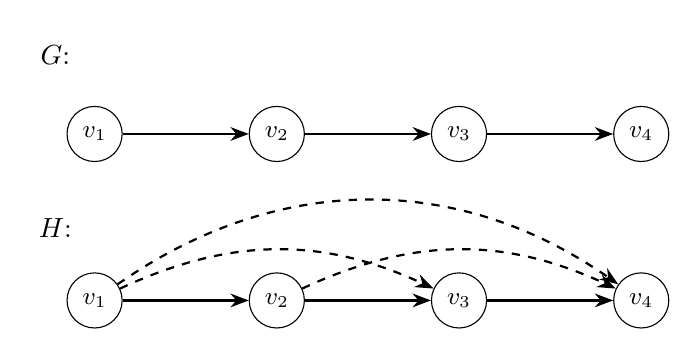
\begin{tikzpicture}[>=Stealth, node distance=1.6cm, every node/.style={circle, draw, minimum size=7mm, inner sep=1pt, font=\small}]
% G
\node[draw=none, font=\normalsize] at (-0.5,1) {$G$:};
\node (v1) {$v_1$};
\node[right=of v1] (v2) {$v_2$};
\node[right=of v2] (v3) {$v_3$};
\node[right=of v3] (v4) {$v_4$};
\draw[->, thick] (v1) -- (v2);
\draw[->, thick] (v2) -- (v3);
\draw[->, thick] (v3) -- (v4);
% H
\node[draw=none, font=\normalsize] at (-0.5,-1.2) {$H$:};
\node[below=1.4cm of v1] (w1) {$v_1$};
\node[right=of w1] (w2) {$v_2$};
\node[right=of w2] (w3) {$v_3$};
\node[right=of w3] (w4) {$v_4$};
\draw[->, thick] (w1) -- (w2);
\draw[->, thick] (w2) -- (w3);
\draw[->, thick] (w3) -- (w4);
\draw[->, thick, dashed] (w1) to[bend left=25] (w3);
\draw[->, thick, dashed] (w1) to[bend left=35] (w4);
\draw[->, thick, dashed] (w2) to[bend left=25] (w4);
\end{tikzpicture}
\end{center}

\begin{algorithm}[H]
\DontPrintSemicolon
\SetKwBlock{Begin}{begin}{}
\Begin{
\textsc{TransitiveClosure}$(G = (V, E))$\;
Compute a topological ordering $v_1, v_2, \ldots, v_n$ of $G$\;
\For{$i \longleftarrow n$ \textbf{down to} $1$}{
    $\mathrm{Reach}[v_i] \longleftarrow$ $n$-bit vector with bit $v_i$ set\;
    \For{\textbf{each} $(v_i, v_j) \in E$}{
        $\mathrm{Reach}[v_i] \longleftarrow \mathrm{Reach}[v_i] \;|\; \mathrm{Reach}[v_j]$\;
    }
}
\Return{$H = \{(u,v) : \text{bit } v \text{ is set in } \mathrm{Reach}[u]\}$}\;
}
\end{algorithm}

\textbf{Correctness:} Processing in reverse topological order ensures $\mathrm{Reach}[v_j]$ is complete before any predecessor $v_i$ reads it (since $i < j$ for every edge $(v_i, v_j)$). After processing $v_i$, $\mathrm{Reach}[v_i]$ contains all vertices reachable from $v_i$.

\textbf{Runtime:} Topological sort $O(m + n)$. Each of $m$ edges triggers one OR of $n$-bit vectors ($O(n)$ each).
\[\boxed{O(mn)}\]


\section*{3. Fault-Tolerant Paths}

\begin{center}
\begin{tikzpicture}[>=Stealth, node distance=1.8cm, every node/.style={circle, draw, minimum size=7mm, inner sep=1pt, font=\small}]
\node (s) {$s$};
\node[above right=0.8cm and 1.5cm of s] (a) {$a$};
\node[below right=0.8cm and 1.5cm of s] (b) {$b$};
\node[right=of a] (c) {$c$};
\node[right=3cm of s, yshift=0cm] (d) {$d$};
\node[above right=0.8cm and 1.5cm of d] (t) {$t$};
\draw[->, thick] (s) -- node[above, draw=none, font=\scriptsize] {$1$} (a);
\draw[->, thick] (s) -- node[below, draw=none, font=\scriptsize] {$1$} (b);
\draw[->, thick] (a) -- node[above, draw=none, font=\scriptsize] {$1$} (c);
\draw[->, thick] (b) -- node[below, draw=none, font=\scriptsize] {$1$} (d);
\draw[->, thick] (c) -- node[above, draw=none, font=\scriptsize] {$1$} (t);
\draw[->, thick] (d) -- node[below right, draw=none, font=\scriptsize] {$1$} (t);
\node[draw=none, below=0.6cm of d, font=\scriptsize] {All capacities $= 1$; two edge-disjoint $s$-$t$ paths};
\end{tikzpicture}
\end{center}

\textbf{Solution 1:}

\textbf{Reduction:} Assign capacity $1$ to every edge. By Menger's theorem, the maximum number of edge-disjoint $s$-$t$ paths equals the max flow from $s$ to $t$ in this unit-capacity network.

\begin{enumerate}[leftmargin=*,itemsep=2pt]
\item Build unit-capacity network on $G$.
\item Run Edmonds-Karp (BFS-based Ford-Fulkerson). Each augmenting path finds one unit of flow.
\item If max flow $\ge 2$: decompose the flow into 2 paths by tracing from $s$ along edges with flow $= 1$ to $t$, removing used edges after each trace.
\item If max flow $< 2$: report no two edge-disjoint $s$-$t$ paths exist.
\end{enumerate}

\textbf{Runtime:} $\le 2$ BFS iterations, each $O(m)$. Flow decomposition: $O(m)$. $\boxed{O(m)}$

\medskip

\textbf{Solution 2:}

\textbf{Reduction:} Assign capacity $1$ to every edge.

\begin{enumerate}[leftmargin=*,itemsep=2pt]
\item Build unit-capacity network on $G$. Initialize flow $f(e) = 0$ for all $e$.
\item \textbf{Repeat up to 2 times:} Run DFS on the residual graph to find an augmenting $s$-$t$ path. If found, push $1$ unit of flow along the path and update the residual graph. If no path exists, stop.
\item If total flow $\ge 2$: decompose into 2 edge-disjoint paths. Else report no two edge-disjoint $s$-$t$ paths exist.
\end{enumerate}

\textbf{Decomposition:} Trace from $s$ along edges with $f(e) = 1$ until $t$; remove used edges; repeat.

\textbf{Correctness:}

$(\Rightarrow)$ $\exists$ two edge-disjoint $s$-$t$ paths $\implies$ send $1$ unit along each $\implies$ feasible flow of value $2$ $\implies$ max flow $\ge 2$.

$(\Leftarrow)$ Max flow $\ge 2$ $\implies$ $\exists$ integer flow with $\forall\, e$: $f(e) \in \{0,1\}$ (integrality theorem). Flow conservation $\implies$ tracing from $s$ along $f{=}1$ edges reaches $t$. Remove first path; remaining flow has value $1$; repeat $\implies$ two edge-disjoint paths.

\textbf{Runtime:} $\le 2$ DFS iterations, each $O(m + n)$. Decomposition: $O(m)$. $\boxed{O(m + n)}$

\vspace{-10pt}
\subsection*{(a)}

Yes. The same reduction generalizes: $k$ edge-disjoint $s$-$t$ paths exist $\iff$ max flow $\ge k$ in the unit-capacity network. Run Ford-Fulkerson for up to $k$ augmenting path iterations.

\vspace{-20pt}
\subsection*{(b)}

$k$ DFS augmenting path iterations $\times$ $O(m + n)$ each $+$ $O(km)$ decomposition.
\[\boxed{O(k(m + n))}\]


\section*{4. Vertex Capacities}

\textbf{Reduction:} Split each vertex $v$ into $v_{\mathrm{in}}$ and $v_{\mathrm{out}}$:

\begin{itemize}[leftmargin=*,itemsep=2pt]
\item All incoming edges of $v$ redirect to $v_{\mathrm{in}}$
\item All outgoing edges of $v$ redirect from $v_{\mathrm{out}}$
\item Add internal edge $(v_{\mathrm{in}}, v_{\mathrm{out}})$ with capacity $c(v)$
\item Original edge $(u, v)$ with capacity $c(e)$ becomes $(u_{\mathrm{out}}, v_{\mathrm{in}})$ with capacity $c(e)$
\end{itemize}

\begin{center}
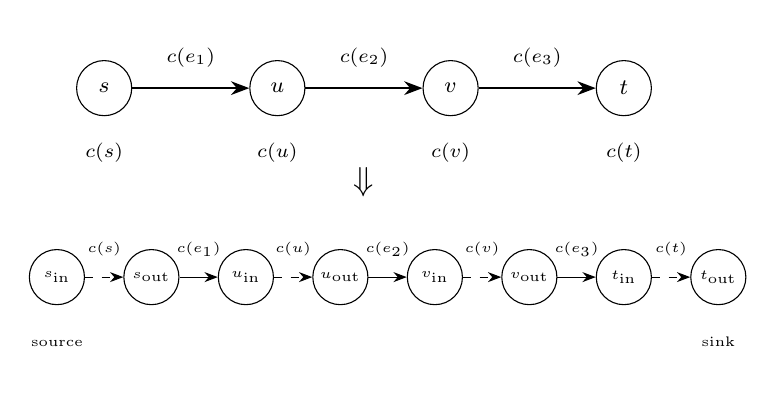
\begin{tikzpicture}[>=Stealth, every node/.style={circle, draw, minimum size=7mm, inner sep=1pt, font=\footnotesize}]
% Original graph
\node (s) at (0,0) {$s$};
\node (u) at (2.2,0) {$u$};
\node (v) at (4.4,0) {$v$};
\node (t) at (6.6,0) {$t$};
\draw[->, thick] (s) -- node[above, draw=none, font=\scriptsize] {$c(e_1)$} (u);
\draw[->, thick] (u) -- node[above, draw=none, font=\scriptsize] {$c(e_2)$} (v);
\draw[->, thick] (v) -- node[above, draw=none, font=\scriptsize] {$c(e_3)$} (t);
\node[draw=none, below=3pt of s, font=\scriptsize] {$c(s)$};
\node[draw=none, below=3pt of u, font=\scriptsize] {$c(u)$};
\node[draw=none, below=3pt of v, font=\scriptsize] {$c(v)$};
\node[draw=none, below=3pt of t, font=\scriptsize] {$c(t)$};
% Arrow
\node[draw=none] at (3.3,-1.2) {\large$\Downarrow$};
% Split graph — use absolute positions to avoid overlap
\node (sin) at (-0.6,-2.4) {\tiny$s_{\text{in}}$};
\node (sout) at (0.6,-2.4) {\tiny$s_{\text{out}}$};
\node (uin) at (1.8,-2.4) {\tiny$u_{\text{in}}$};
\node (uout) at (3.0,-2.4) {\tiny$u_{\text{out}}$};
\node (vin) at (4.2,-2.4) {\tiny$v_{\text{in}}$};
\node (vout) at (5.4,-2.4) {\tiny$v_{\text{out}}$};
\node (tin) at (6.6,-2.4) {\tiny$t_{\text{in}}$};
\node (tout) at (7.8,-2.4) {\tiny$t_{\text{out}}$};
\draw[->, dashed] (sin) -- node[above, draw=none, font=\tiny] {$c(s)$} (sout);
\draw[->] (sout) -- node[above, draw=none, font=\tiny] {$c(e_1)$} (uin);
\draw[->, dashed] (uin) -- node[above, draw=none, font=\tiny] {$c(u)$} (uout);
\draw[->] (uout) -- node[above, draw=none, font=\tiny] {$c(e_2)$} (vin);
\draw[->, dashed] (vin) -- node[above, draw=none, font=\tiny] {$c(v)$} (vout);
\draw[->] (vout) -- node[above, draw=none, font=\tiny] {$c(e_3)$} (tin);
\draw[->, dashed] (tin) -- node[above, draw=none, font=\tiny] {$c(t)$} (tout);
\node[draw=none, below=3pt of sin, font=\tiny] {source};
\node[draw=none, below=3pt of tout, font=\tiny] {sink};
\end{tikzpicture}
\end{center}

New source $= s_{\mathrm{in}}$, new sink $= t_{\mathrm{out}}$. The new graph $G'$ has $2n$ vertices and $m + n$ edges.

\textbf{Correctness:}

$(\Rightarrow)$ Given a feasible flow $f'$ in $G'$, define $f(u,v) = f'(u_{\mathrm{out}}, v_{\mathrm{in}})$ in $G$. Edge capacities are preserved. The total flow through $v$ equals $f'(v_{\mathrm{in}}, v_{\mathrm{out}}) \le c(v)$, so the vertex capacity is satisfied.

$(\Leftarrow)$ Given a feasible flow $f$ in $G$ with vertex capacities, define:
\[
f'(u_{\mathrm{out}}, v_{\mathrm{in}}) = f(u,v), \qquad f'(v_{\mathrm{in}}, v_{\mathrm{out}}) = \textstyle\sum_{u} f(u,v)
\]
Since $f$ respects $c(v)$: $f'(v_{\mathrm{in}}, v_{\mathrm{out}}) \le c(v)$. Conservation in $G'$ follows from conservation in $G$.

$\implies$ Max flow in $G'$ = max flow in $G$ with vertex capacities. Run any max-flow algorithm on $G'$. \qed

\[\boxed{\text{Reduce to standard max-flow on } G' \text{ with } 2n \text{ vertices, } m + n \text{ edges}}\]


\section*{5. Convex Combination of Flows}

\begin{center}
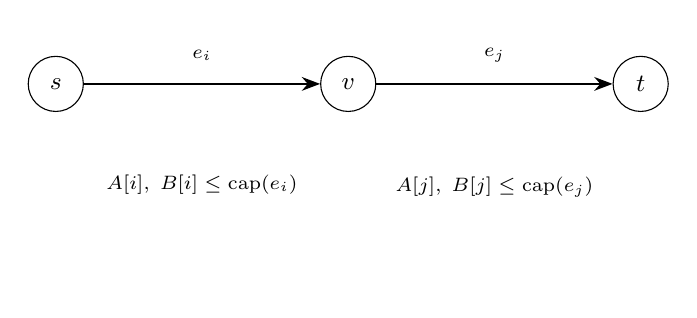
\begin{tikzpicture}[>=Stealth, node distance=3cm, every node/.style={circle, draw, minimum size=7mm, inner sep=1pt, font=\small}]
\node (s) {$s$};
\node[right=of s] (u) {$v$};
\node[right=of u] (t) {$t$};
\draw[->, thick] (s) -- node[above, draw=none, font=\scriptsize] {$e_i$} node[below, draw=none, font=\scriptsize] {$A[i],\; B[i] \le \mathrm{cap}(e_i)$} (u);
\draw[->, thick] (u) -- node[above, draw=none, font=\scriptsize] {$e_j$} node[below, draw=none, font=\scriptsize] {$A[j],\; B[j] \le \mathrm{cap}(e_j)$} (t);
\end{tikzpicture}
\end{center}

Let $f_1$, $f_2$ be feasible flows with arrays $A[1..m]$, $B[1..m]$. Define $C[i] = c \cdot A[i] + (1 - c) \cdot B[i]$ for $0 \le c \le 1$.

\textbf{Capacity constraints:} Since $c \ge 0$, $1 - c \ge 0$, $A[i] \ge 0$, $B[i] \ge 0$:
\[
C[i] = c \cdot A[i] + (1-c) \cdot B[i] \ge 0
\]
Since $A[i] \le \mathrm{cap}(e_i)$ and $B[i] \le \mathrm{cap}(e_i)$:
\[
C[i] \le c \cdot \mathrm{cap}(e_i) + (1-c) \cdot \mathrm{cap}(e_i) = \mathrm{cap}(e_i)
\]

\textbf{Flow conservation:} For each vertex $v \ne s, t$:
\begin{align*}
\sum_{\text{in}} C[i] - \sum_{\text{out}} C[i]
&= c\!\left(\sum_{\text{in}} A[i] - \sum_{\text{out}} A[i]\right) + (1-c)\!\left(\sum_{\text{in}} B[i] - \sum_{\text{out}} B[i]\right) \\
&= c \cdot 0 + (1-c) \cdot 0 = 0
\end{align*}

$\implies C[1..m]$ satisfies capacity constraints and flow conservation $\implies C$ is a feasible flow. \qed

\[\boxed{|f_C| = c \cdot |f_1| + (1-c) \cdot |f_2|}\]


\end{document}
